\documentclass[a4paper,11pt]{article}
\usepackage[french]{babel}
\usepackage[utf8]{inputenc}
\usepackage[left=2.5cm,top=2cm,right=2.5cm,nohead,nofoot]{geometry}
\usepackage{url}
\usepackage{graphicx}
\usepackage{float}
\usepackage[colorinlistoftodos]{todonotes}
\usepackage{hyperref}

\linespread{1.1}

%\setcounter{section}{-1}

\begin{document}

\begin{titlepage}
\begin{center}
\textbf{\textsc{UNIVERSIT\'E DE MONTR\'EAL}}\\
%\textbf{\textsc{Faculté des Sciences}}\\
%\textbf{\textsc{Département d'Informatique}}
\vfill{}\vfill{}
\begin{center}{\Huge Rapport : TP2 - Classification de textes}\end{center}{\Huge \par}
\begin{center}{\large Pierre Gérard}\end{center}{\Huge \par}
\vfill{}\vfill{} \vfill{}
\begin{center}{\large \textbf{IFT 3335 Intelligence artificielle: Introduction}}\hfill{\\Jian-Yun Nie, William Lechelle}\end{center}{\large\par}
\vfill{}\vfill{}\enlargethispage{3cm}
\textbf{Année académique 2015~-~2016}
\end{center}
\end{titlepage}

%\begin{abstract}
%Ce rapport présente ...
%\end{abstract}


\tableofcontents

\pagebreak

\section{Base}

\section{Selection d'attributs}

\todo{Pourquoi la selection}

\subsection{Résultats expérimentaux}

\begin{figure}[H]
	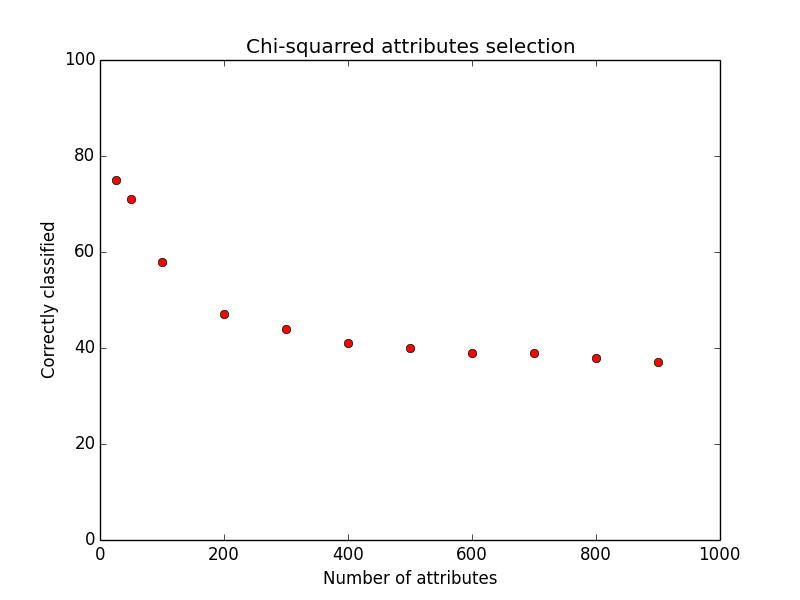
\includegraphics[width=12cm]{images/part2chisq.png} 
	\centering
	\caption{Res}
	\label{fig:comp}
\end{figure}


\subsection{Discussion et menaces à la validité}

Si on prend trop de donné, ça met du temps.

Si on prend trop de donné, on a du “bruit” qui menace notre apprentissage
Si on en prends pas assez, on a une “perte d’information” essentielle.

Attention, pas cable de généralisé

\section{Stemming}

\todo{Pourquoi le stemming}

\subsection{Résultats expérimentaux}

Pour tester l'utilité du stemming, réalisons une expérience empirique pour différents algorithme et nombre d'attributs retenu et cela pour les deux ensembles de données.

Regardons le pourcentage d'éléments bien classifié:
\begin{center}
\begin{tabular}{ |c|c|c| } 
 \hline
  & Sans stemming & Avec stemming \\ 
 \hline
 Ohsumed NaiveBayes 1000 attributs 10-fold  & 35.6\% & 37.9\% \\ 
 Ohsumed NaiveBayes 300 attributs 10-fold  & 44.1\% & 45.4\% \\ 
 Ohsumed J48 300 attributs 3-fold & 76.4\% & 77.5\% \\ 
 Ohsumed AdaBoost 300 attributs 10-fold & 62.5\% & 66.9\% \\
 \hline
 Reuters NaiveBayes 1000 attributs 10-fold & 79.3\% & 79.7\% \\
 Reuters NaiveBayes 300 attributs 10-fold  & 78.6\% & 78.5\% \\ 
 Reuters J48 300 attributs 3-fold & 87.4\% & 86.9\% \\ 
 Reuters AdaBoost 300 attributs 10-fold & 70.1\% & 70.1\% \\ 
 Reuters AdaBoost 1000 attributs 10-fold & 70.0\% & 70.0\% \\ 
 \hline
\end{tabular}
\end{center}

Pour Ohsumed, on remarque que, dans la plupart des cas, le nombre d'attribut bien classifié augmente lorsqu'on utilise la technique de stemming. 

Pour Reuters, on remarque que le stemming n'a pas grande influence sur les résultats.
\subsection{Discussion}

Sans grande surprise, ..

\section{Evaluation des algos}

\subsection{Résultats expérimentaux}

\begin{center}
\begin{tabular}{ |c|c|c| } 
 \hline
  & Reuters &  Ohsumed\\ 
 \hline
 NaiveBayes 1000 attributs 10-fold  & 35.6\% & 37.9\% \\  
 \hline
\end{tabular}
\end{center}

\subsection{Discussion}


\section{Exploration}

%\section{Introduction}

%\section{Etat de l'art}

%\section{Méthode expérimentale}

%\section{Résultats expérimentaux}

%\section{Discussion}

%\section{Conclusion}

\end{document}
